\chapter{Advisor}
%ILP - integer linear programming

To support performance-aware migration between ORM frameworks, \emph{ORMorpher} integrates an optimization module that selects the most suitable ORM framework, or a combination of frameworks, for executing a given query workload under specified resource constraints. This task is inherently non-trivial, as ORM frameworks exhibit different runtime behaviors and memory characteristics depending on the query structure,  and entity complexity. While syntactic translation ensures semantic equivalence across frameworks, optimal performance requires systematic selection based on empirical evidence and formal reasoning. \emph{ORMorpher} addresses this challenge by formulating the ORM framework selection problem as an instance of \emph{Integer Linear Programming} (ILP), enabling the derivation of optimal configurations with respect to execution time, memory usage, and user-defined limits. %This integration enables \emph{ORMorpher} to provide not only syntactically valid translations, but also \emph{data-driven and constraint-aware recommendations} for ORM framework selection, tailored to practical deployment requirements.

\section{What-if analysis}

Prior to optimization, \emph{ORMorpher} performs a \emph{what-if analysis} to collect detailed performance metrics. This phase executes all input queries, defined over all candidate frameworks including original ORM representations, against a common underlying DBMS. For each query-framework pair, the system measures runtime and memory consumption. These metrics, together with query frequency weights and user constraints (e.g., memory budget or number of frameworks allowed), serve as inputs to the ILP model. The goal is to minimize the total weighted execution cost of the workload, while ensuring that the selected configuration respects user-imposed limitations.

\section{ILP formulation}

Formally, let $W$ be the set of queries and $F$ the set of ORM frameworks. For each query $q \in W$, its relative importance is captured by a frequency parameter $z_q$. Empirical measurements yield $\text{cost}(q, f)$, the runtime of query $q$ on framework $f$, and $\text{mem}(q, f)$, the corresponding memory usage. The global memory constraint is denoted $\text{MEM}$, and the upper bound on the number of frameworks to be used is given by $N$. Decision variables $x_{q,f} \in \{0,1\}$ indicate whether query $q$ is assigned to framework $f$, and $y_f \in \{0,1\}$ indicates whether framework $f$ is selected.

The optimization objective is to minimize the total weighted cost:
$$\min \sum_{q \in W} \sum_{f \in F} z_q \cdot \text{cost}(q, f) \cdot x_{q,f}$$

\noindent
subject to the following constraints:
\begin{align*}
&\sum_{f \in F} y_f \leq N && \text{(Select at most $N$ frameworks)} \\
&\sum_{f \in F} x_{q,f} = 1 && \forall q \in W \quad \text{(Each query uses one framework)} \\
&x_{q,f} \leq y_f && \forall q \in W,\ \forall f \in F \quad \text{(Query uses only selected frameworks)} \\
&\sum_{q \in W} \sum_{f \in F} \text{mem}(q,f) \cdot x_{q,f} \leq \text{MEM} && \text{(Memory constraint)}
\end{align*}

These constraints ensure that (1) no more than $N$ frameworks are selected, (2-3) each query is evaluated using exactly one selected framework, and (4) the total memory usage remains within the allowed budget.

The resulting ILP instance is solved using an off-the-shelf solver such as \emph{Gurobi}, which searches the feasible solution space and returns an assignment of queries to frameworks that minimizes the objective while satisfying all constraints.

\begin{figure}
\centering
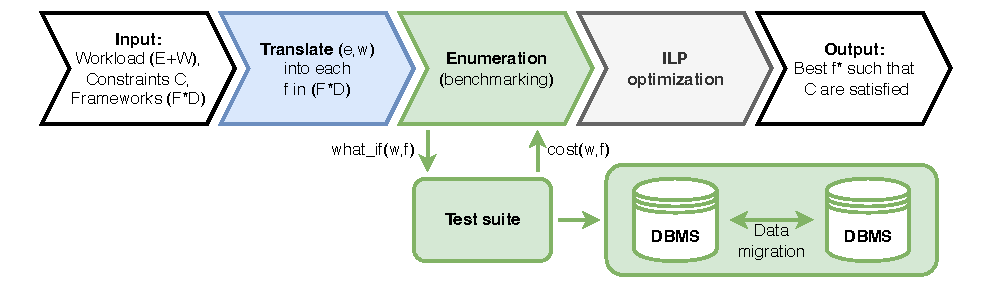
\includegraphics[scale=0.8]{thesis/img/thesis/ORM-workflow.pdf}
\caption{TODO: Workflow }
\label{fig:workflow}
\end{figure}

\afterpage{
\begin{landscape}
\begin{figure}[p]
\centering
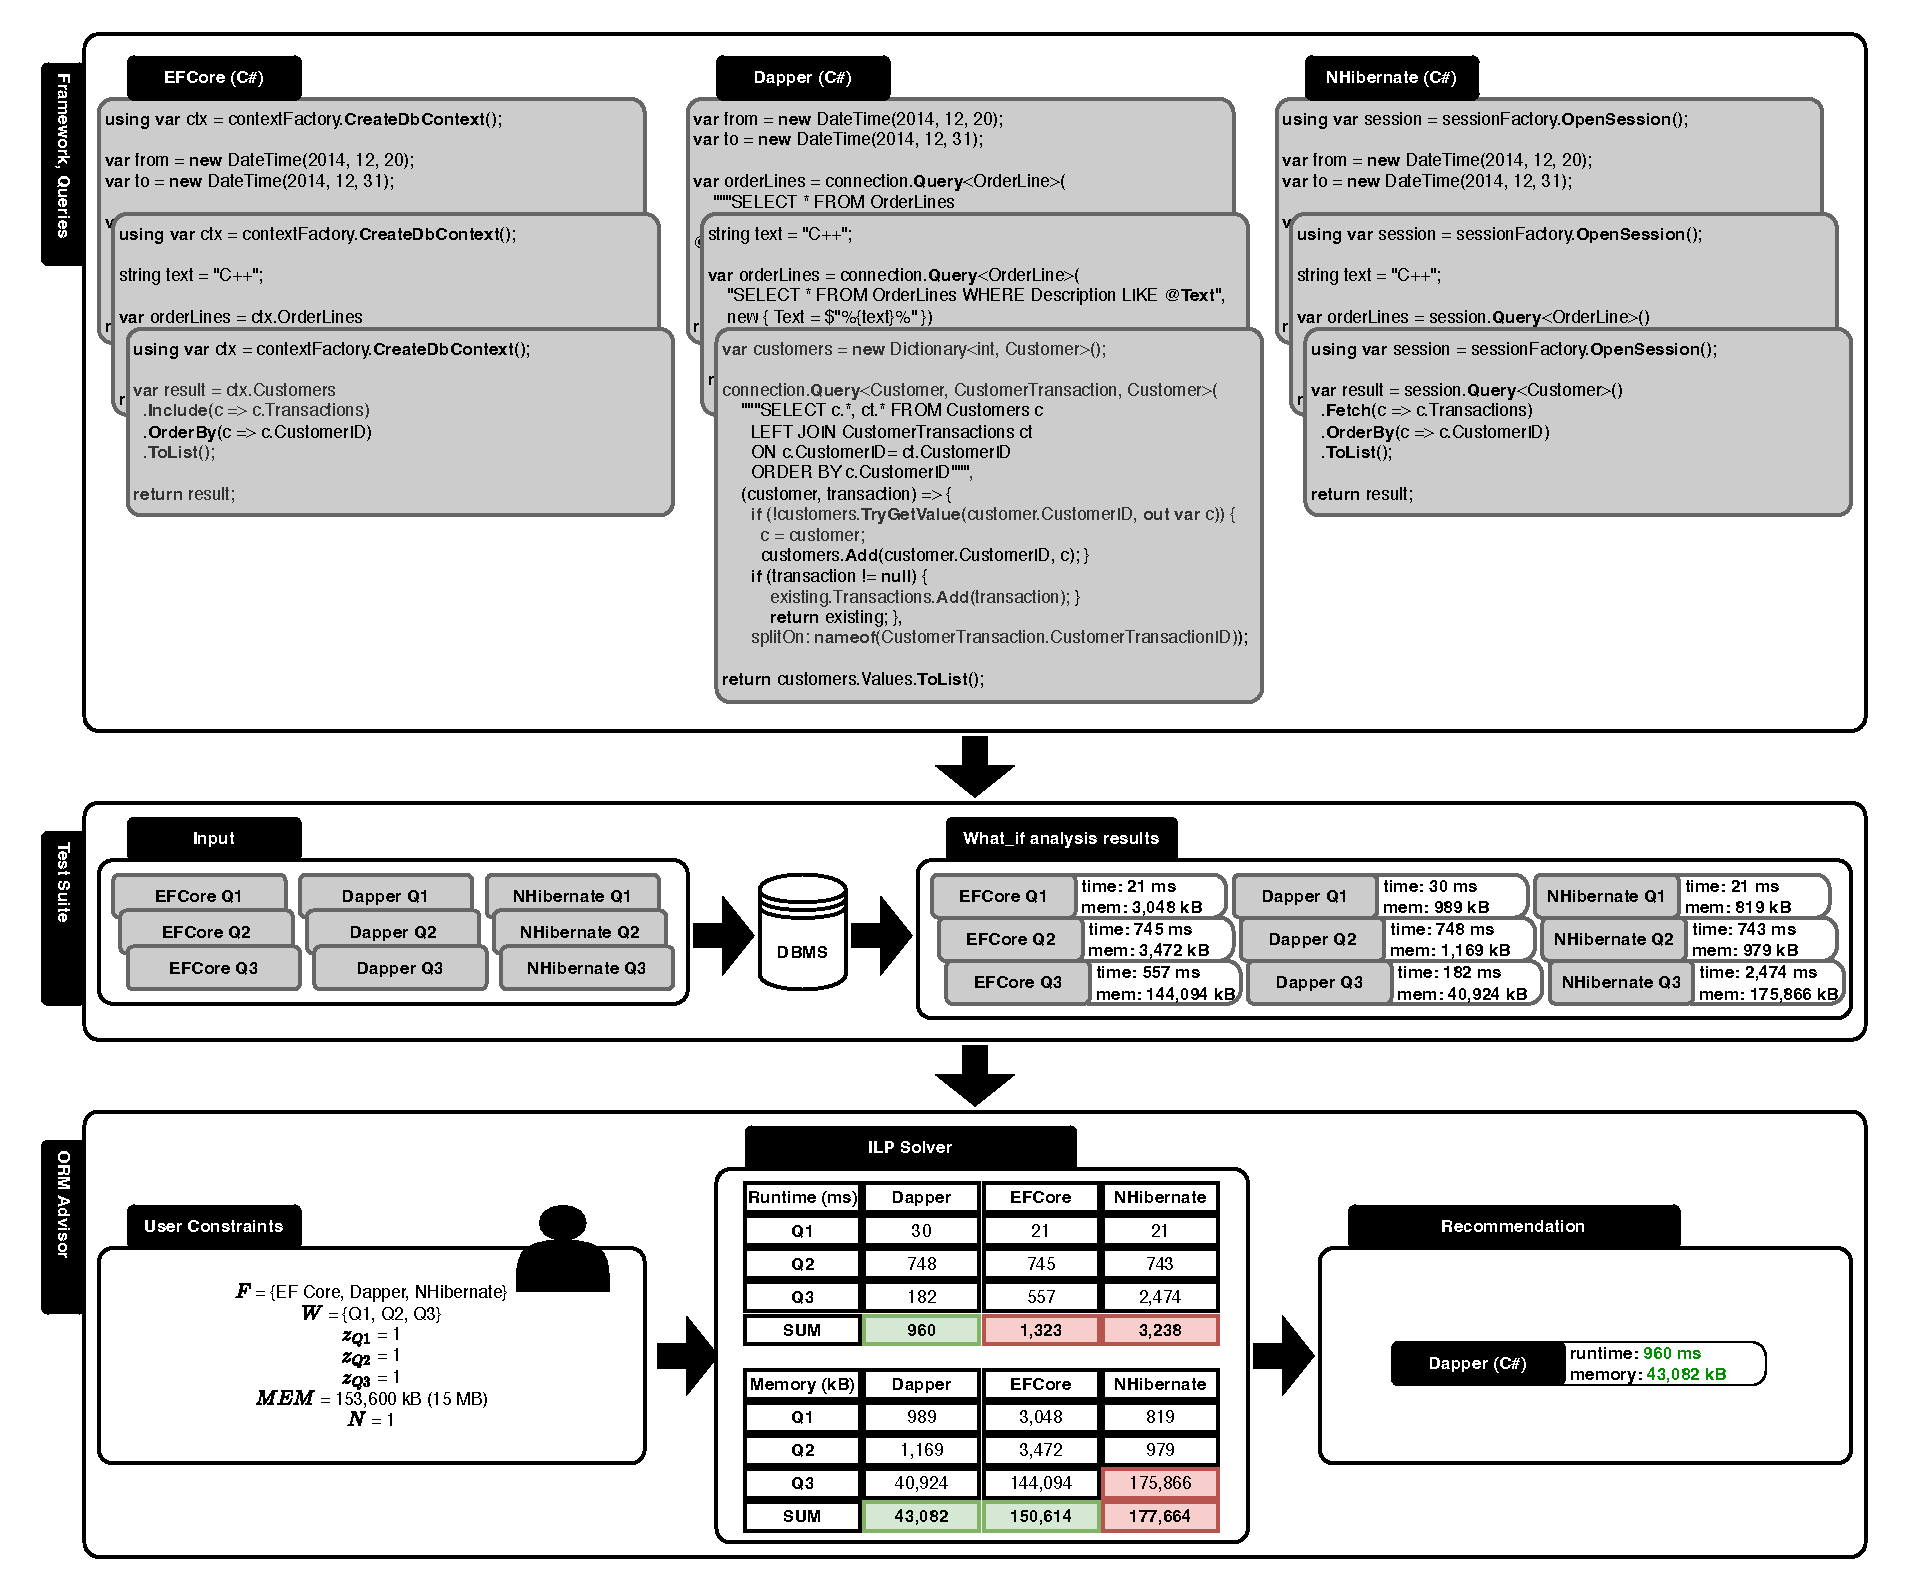
\includegraphics[width=\textwidth]{thesis/img/thesis/ORM-example.pdf}
\caption{TODO: Workflow illustrated using running example, translation from EFCore to optimal framework (Dapper in this case)}
\label{fig:example}
\end{figure}    
\end{landscape}
}

\begin{example}    
\small
Figure~\ref{fig:example} illustrates a complete workflow of how \emph{ORMorpher} operates. The user specifies the input ORM framework (e.g., EFCore) and provides entity mappings for \texttt{Customer} and \texttt{CustomerTransaction}, along with two queries, \textbf{Q1} and \textbf{Q2}. The user also selects Dapper and NHibernate as target frameworks. ORMorpher first translates the input into an intermediate representation (Step 2), and then generates target-specific code via \texttt{buildClass()} and \texttt{build()}/\texttt{buildRawSQL()} methods. For NHibernate, additional metadata must be retrieved from the underlying DBMS to complete the translation (Step 3). The generated outputs are made available for inspection (Step 4). A what-if analysis is then performed using a query test suite executed on the DBMS (Step 5), evaluating runtime and memory usage for all queries across source and translated frameworks (Step 6). Given user-defined constraints, such as memory limits and maximum number of frameworks (Step 7), an ILP solver is invoked (Step 8) to find the optimal framework configuration that minimizes runtime (Step 9), producing the final recommendation (Step 10).
\qed
\end{example}


\begin{figure}
\centering
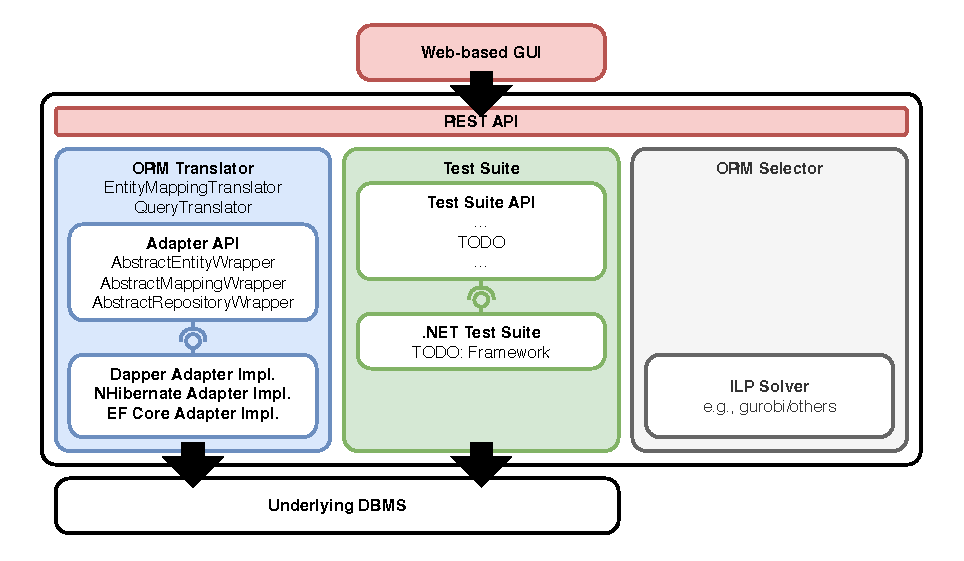
\includegraphics[scale=0.8]{thesis/img/thesis/ORM-architecture.pdf}
\caption{TODO: Architecture}
\label{fig:architecture}
\end{figure}

\section{Extensions}

...